\documentclass[14pt,a4paper]{scrartcl}
\usepackage[utf8]{inputenc}
\usepackage{ragged2e}
\usepackage[english,russian]{babel}
\usepackage{misccorr,color,ragged2e,amsfonts,
amsthm,graphicx,systeme,amsmath,mdframed,lipsum}


% Default fixed font does not support bold face
\DeclareFixedFont{\ttb}{T1}{txtt}{bx}{n}{12} % for bold
\DeclareFixedFont{\ttm}{T1}{txtt}{m}{n}{12}  % for normal

% Custom colors
\usepackage{color}
\definecolor{deepblue}{rgb}{0,0,0.5}
\definecolor{deepred}{rgb}{0.6,0,0}
\definecolor{deepgreen}{rgb}{0,0.5,0}

\usepackage{listings}
\usepackage{slashbox}
\usepackage{titling}
\usepackage{float}
\usepackage{picture}
\usepackage{cancel}
\usepackage{multicol}
\usepackage{wrapfig}

\usepackage{pgfplots}
\usepgflibrary{shapes.geometric}
\usetikzlibrary{calc}
\pgfplotsset{my style/.append style={axis x line=middle, axis y line=middle, xlabel={$x$}, ylabel={$y$}, axis equal}}
\pgfplotsset{my style 2/.append style={axis x line=middle, axis y line=middle, xlabel={$x$}}}
\usepgfplotslibrary{fillbetween}



\begin{document}
  \begin{titlepage}
    \begin{center}
      \textbf{МІНІСТЕРСТВО ОСВІТИ І НАУКИ УКРАЇНИ\\
      НАВЧАЛЬНО-НАУКОВИЙ КОМПЛЕКС\\
      ``ІНСТИТУТ ПРИКЛАДНОГО СИСТЕМНОГО АНАЛІЗУ''\\
      НАЦІОНАЛЬНОГО ТЕХНІЧНОГО УНІВЕРСИТЕТУ УКРАЇНИ\\
      ``КИЇВСЬКИЙ ПОЛІТЕХНІЧНИЙ ІНСТИТУТ''}


      \vspace{1.5cm}
      РОЗРАХУНКОВА ГРАФІЧНА РОБОТА\\
      З КУРСУ "МАТЕМАТИЧА СТАТИСТИКА"\\
      Варіант: 104

      \vspace{5cm}

      \begin{flushright}
        Виконав:\\
        Вітковськй~Д.О.\\
        \vspace{3mm}
        Прийняв:\\
        Ільєнко~А.Б.
      \end{flushright}

      \vfill

      Київ - 2021
    \end{center}
  \end{titlepage}

\def\be{\begin{equation}} % Рівняння
\def\ee{\end{equation}}
\def\D{\mathbb{D}}
\def\E{\mathbb{E}}

\renewcommand{\contentsname}{Зміст}
\tableofcontents

\newpage
\textbf{Завдання.}\\
\begin{enumerate}
  \item Провести первинний аналіз вибірки. Це включає статистичний ряд, емпіричну функцію розподілу, її графік, полігон частот, гістограму, box-and-whiskers plot.
  \item Знайти вибіркове середнє, вибіркову дисперсію, виправлену вибіркову дисперсію, вибіркову медіану, вибіркову моду, вибіркові коефіцієнти асиметрії та ексцесу.
  \item \underline{Обґрунтувати} та висунути (нову) гіпотезу про розподіл генеральної сукупності.
  \item Методом моментів та методом максимальної вірогідності знайти оцінки параметрів розподілу.
  \item Для кожного з параметрів кращу з цих двох оцінок перевірити на (асимптотичну незміщеність), консистентність та ефективність.
  \item Побудувати довірчі інтервали надійністю 0.95 для параметрів розподілу.
  \item Перевірити висунуту гіпотезу про розподіл генеральної сукупності за допомогою критерію $\chi^2$. Якщо гіпотеза суперечить вибірковим даним, перейти до п.~3.
  \item Зробити висновки.
\end{enumerate}
\newpage

Вихідна реалізація вибірки:\\\\
\begin{tabular}{r r r r r r r r r r}
-1.66 & -0.10 & 2.84 & 5.04 & 1.60 & -2.80 & -0.72 & 5.47 & -4.20 & 0.67\\
-2.49 & -2.40 & 5.99 & -3.26 & 2.16 & 0.51 & -3.49 & 5.10 & -1.24 & 2.58\\
-1.06 & -0.84 & 4.09 & 6.54 & -2.96 & 6.77 & 7.29 & -2.87 & 2.29 & 1.37\\
2.51 & 1.67 & -4.48 & -1.46 & 0.84 & -2.01 & -1.07 & 0.01 & -4.33 & 3.41\\
0.49 & -3.41 & 9.65 & -3.84 & 6.15 & 8.17 & -1.55 & -3.60 & -2.73 & \textbf{18.49}\\
1.38 & 6.09 & -2.15 & 9.68 & -0.47 & 7.67 & -1.47 & 3.30 & 4.58 & 0.43\\
2.19 & 5.19 & 1.95 & -4.44 & -0.22 & \textbf{-4.49} & -3.06 & 1.09 & -1.03 & -1.18\\
3.52 & 2.15 & -3.48 & 3.64 & -3.21 & -0.82 & -3.29 & -2.09 & 2.81 & -0.92\\
0.24 & 1.39 & -4.22 & 1.20 & -2.68 & -1.93 & 1.49 & -3.64 & 1.58 & 1.59\\
0.66 & -2.04 & 3.41 & 2.69 & 3.73 & -2.11 & 4.02 & -0.66 & 1.25 & -3.07
\end{tabular}\\\\

Відсортована реалізація вибірки:\\\\
\begin{tabular}{r r r r r r r r r r}
-4.49 & -4.48 & -4.44 & -4.33 & -4.22 & -4.20 & -3.84 & -3.64 & -3.60 & -3.49\\
-3.48 & -3.41 & -3.29 & -3.26 & -3.21 & -3.07 & -3.06 & -2.96 & -2.87 & -2.80\\
-2.73 & -2.68 & -2.49 & -2.40 & -2.15 & -2.11 & -2.09 & -2.04 & -2.01 & -1.93\\
-1.66 & -1.55 & -1.47 & -1.46 & -1.24 & -1.18 & -1.07 & -1.06 & -1.03 & -0.92\\
-0.84 & -0.82 & -0.72 & -0.66 & -0.47 & -0.22 & -0.1 & 0.01 & 0.24 & 0.43\\
0.49 & 0.51 & 0.66 & 0.67 & 0.84 & 1.09 & 1.20 & 1.25 & 1.37 & 1.38\\
1.39 & 1.49 & 1.58 & 1.59 & 1.60 & 1.67 & 1.95 & 2.15 & 2.16 & 2.19\\
2.29 & 2.51 & 2.58 & 2.69 & 2.81 & 2.84 & 3.30 & 3.41 & 3.41 & 3.52\\
3.64 & 3.73 & 4.02 & 4.09 & 4.58 & 5.04 & 5.10 & 5.19 & 5.47 & 5.99\\
6.09 & 6.15 & 6.54 & 6.77 & 7.29 & 7.67 & 8.17 & 9.65 & 9.68 & 18.49
\end{tabular}\newpage


\section{Первинний аналіз вибірки.}
\quadОскільки з даних видно, що розподіл неперервний, то для побудови статистичного ряду дані з вибірки треба розбити на рівновеликі інтервали. Емпіричною формулою кількості таких інтервалів є формула Стерджеса:
\be m = 1 + \log_2{n} = 1 + \log_2{100}=7.644\approx8.\ee

Але мені така кількість видається замалою, тому використаю значення
\be m=12. \ee
Отже\\
$x_{min}=\min\{x\} = -4.49;$\\
$x_{max}=\max\{x\} = 18.49.$\\
Розмах вибірки\\
$R = x_{max}-x_{min} = 22.98.$\\
Таким чином довжина кроку дорівнює $1.915$.
\vspace{3cm}
\begin{table}[H]
  \centering
  \begin{tabular}{|c||c|c|c|c|}\hline
    \parbox[c][0.8cm]{Iнтервал} & $[-4.49, -2.575)$ & $[-2.575, -0.66)$ & $[-0.66, 1.255)$ & $[1.255, 3.17)$ \\\hline\hline
    \parbox[c][1.4cm]{3cm}{\centeringСередина\\інтервалу} & $-3.525$ & $-1.6175$ & $0.2975$ & $4.425$\\\hline
    Частота & 22 & 21 & 15 & 18 \\\hline
    \parbox[c][1.4cm]{3cm}{\centeringКумулятивна\\частота} & 22 & 43 & 58 & 76 \\\hline
    \parbox[c][1.4cm]{3cm}{\centeringВідносна\\частота} & $0.22$ & $0.21$ & $0.15$ & $0.18$ \\\hline
    \parbox[c][1.8cm]{3cm}{\centeringКумулятивна\\відносна\\частота} & $0.22$ & $0.43$ & $0.58$ & $0.76$ \\\hline
  \end{tabular}\caption{Статистичний ряд.}
\end{table}
\newpage
\begin{table}[H]
  \centering
  \begin{tabular}{|c||c|c|c|c|}\hline
    \parbox[c][0.8cm]{Iнтервал} & $[3.17, 5.085)$ & $[5.085, 7)$ & $[7, 8.915)$ & $[8.915, 10.83)$ \\\hline\hline
    \parbox[c][1.4cm]{3cm}{\centeringСередина\\інтервалу} & $4.1275$ & $6.0425$ & $7.9575$ & $9.8725$ \\\hline
    Частота & 10 & 8 & 3 & 2 \\\hline
    \parbox[c][1.4cm]{3cm}{\centeringКумулятивна\\частота} & 86 & 94 & 97 & 99 \\\hline
    \parbox[c][1.4cm]{3cm}{\centeringВідносна\\частота} & $0.1$ & $0.08$ & $0.03$ & $0.02$ \\\hline
    \parbox[c][1.8cm]{3cm}{\centeringКумулятивна\\відносна\\частота} & $0.86$ & $0.91$ & $0.97$ & $0.99$ \\\hline
  \end{tabular}\\
  \vspace{0.8cm}
  \begin{tabular}{|c||c|c|c|c|}\hline
    \parbox[c][0.8cm]{Iнтервал} & $[10.83, 12.745)$ & $[12.745, 14.66)$ & $[14.66, 16.575)$ & $[16.575, 18.49]$ \\\hline\hline
    \parbox[c][1.4cm]{3cm}{\centeringСередина\\інтервалу} & $11.7875$ & $13.7025$ & $15.6175$ & $17.5325$ \\\hline
    Частота & 0 & 0 & 0 & 1 \\\hline
    \parbox[c][1.4cm]{3cm}{\centeringКумулятивна\\частота} & 99 & 99 & 99 & 100 \\\hline
    \parbox[c][1.4cm]{3cm}{\centeringВідносна\\частота} & 0 & 0 & 0 & $0.01$ \\\hline
    \parbox[c][1.8cm]{3cm}{\centeringКумулятивна\\відносна\\частота} & $0.99$ & $0.99$ & $0.99$ & 1 \\\hline
  \end{tabular}
  \caption{Статистичний ряд (продовження).}
\end{table}
\\Емпірична функція розподілу (інтервальна):\\
\be
F_n^*(x)=\left\{\begin{array}{ll}
  0, & x < x_0^*;\\
  \omega_k^\text{кумул}, & x_k^*\leq x < x_{k+1}^*.
\end{array}\right.
\ee
, де $x_k^*$~--~початок k-того інтервалу, кінець (k-1)-го, а  $\omega_k^\text{кумул}$~--~кумулятивна відносна частота для k-того інтервалу.\newpage
Відповідна функція для даного інтервального розбиття:
\be
F_n^*(x)=\left\{\begin{array}{ll}
  0, & x < -4.49;\\
  0.22, & x\in[-4.49, -2.575);\\
  0.43, & x\in[-2.575, -0.66);\\
  0.58, & x\in[-0.66, 1.255);\\
  0.76, & x\in[1.255, 3.17);\\
  0.86, & x\in[3.17, 5.085);\\
  0.91, & x\in[5.085, 7);\\
  0.97, & x\in[7, 8.915);\\
  0.99, & x\in[8.915, 16.575);\\
  1, & x\geq 16.575.
\end{array}\right.
\ee\\
Її графік:
\begin{center}
  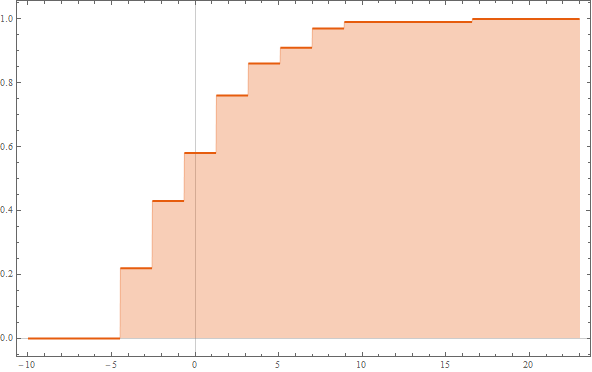
\includegraphics[scale=0.85]{РР2 емп. ф-ція розподілу.png}\\
  \caption{Рис. 1. Інтервальна емпірична функція розподілу.}
\end{center}
\newpage
Гістограма за заданими інтервалами:
\begin{center}
  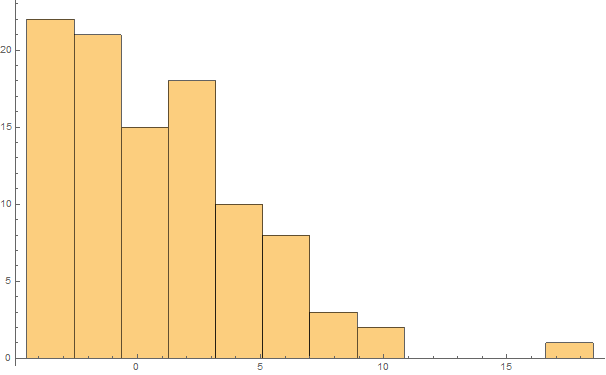
\includegraphics[scale=0.85]{РР2 гістограма.png}\\
  \caption{Рис. 2. Гістограма розподілу.}
\end{center}
\newpage
Для побудови графіку "ящик з вусами" використано значення, обчислені у наступному розділі, а саме: вибіркове середнє, медіану, перший та третій квартилі і мінімум та максимум як значення кінців вусів.
\begin{center}
  \includegraphics[scale=0.85]{РР2 box plot}\\
  \caption{Рис. 3. Ящик з вусами.}
\end{center}
\newpage
\section{Знаходження описових статистик.}
\underline{Вибіркове середнє:}
\be
  \overline{x}=\frac1n\sum\limits_{i=1}^n x_i=
  \frac1{100}\sum\limits_{i=1}^{100}x_i=0.7938
\ee
\underline{Вибіркова дисперсія:}
\be
  s^2=\D _\xi^{**}=
  \frac1n\sum\limits_{i=1}^n(x_i-\overline{x})^2=
  \frac1{100}\sum\limits_{i=1}^{100}(x_i-0.7938)^2=15.0129
\ee
\underline{Виправлена вибіркова дисперсія:}
\be
  s_0^2=\D _\xi^{***}=
  \frac1{n-1}\sum\limits_{i=1}^n(x_i-\overline{x})^2=
  \frac1{99}\sum\limits_{i=1}^{100}(x_i-0.7938)^2=15.1645
\ee
\underline{Вибіркова медіана:}\\

Оскільки маємо відсортований набір усіх $x$, можна доволі легко обчислити медіану за наступною формулою:
$$\mathcal{M}^*_e=
\left\{\begin{array}{ll}
  x_{(k+1)}, & n=2k+1\\
  \frac{x_{(k)}+x_{(k+1)}}2, & n=2k
\end{array}\right.$$
, де $k\in\mathbb{N}$\\
Тоді у нашому випаддку медіана обчислюється наступним чином:
\be
  \mathcal{M}^*_e=\frac{x_{(k)}+x_{(k+1)}}2=\frac{0.43+0.49}2=
  0.46
\ee
\underline{Вибіркова мода:}
\be
  mo = 1 \text{--- номер модального класу}
\ee
\be
  \mathcal{M}^*_o=y_{mo-1}+(y_{mo}-y_{mo-1})\cdot
  \frac{n_{mo}-n_{mo-1}}{(n_{mo}-n_{mo-1})+(n_{mo}-n_{mo+1})}\fbox{=}
\ee
, де $y_{mo-1}$, $y_{mo}$ – вiдповiдно нижня та верхня межi модального класу; $n_{mo}$, $n_{mo-1}$, $n_{mo+1}$ –
частоти вiдповiдно модального, передмодального та пiслямодального iнтервалiв.\newpage
$$
  \fbox{=}-4.49+(-2.575-(-4.49))\cdot
  \frac{22-0}{(22-0)+(22-21)} = -2.65826
$$
\underline{Вибіркові коефіцієнти асиметрії та екцесу:}\\

Для знаходження цих коефіцієнтів потрібно обчислювати вибіркові центральні моменти за наступною формулою:
\be
  \overline{\mu_k}=\frac1n\sum\limits_{i=1}^n(x_i-\overline{x})^k
\ee
\underline{Вибірковий коефіцієнт асиметрії:}
\be
  As = \frac{\overline{\mu_3}}{s_0^3}=
  \frac{\frac1{100}\sum\limits_{i=1}^{100}(x_i-\overline{x})^3}{\left(\D ^{***}_\xi\right)^\frac32}=
  1.22459
\ee
\underline{Вибірковий коефіцієнт ексцесу:}
\be
  Ek = \frac{\overline{\mu_4}}{s_0^4}-3=
  \frac{\frac1{100}\sum\limits_{i=1}^{100}(x_i-\overline{x})^4}{\left(\D ^{***}_\xi\right)^2}-3=
  2.822
\ee
\underline{Перший квартиль:}
$$\alpha=0.25\Rightarrow
K = n\cdot\alpha=100*0.25=25\in\mathbb{Z}\Rightarrow$$
\be\Rightarrow Q_1=q_\alpha=\frac{x_{(K)}+x_{(K+1)}}2=\frac{-2.15-2.11}2=-2.13\ee
\underline{Третій квартиль:}
$$\alpha=0.75\Rightarrow
K = n\cdot\alpha=100*0.75=75\in\mathbb{Z}\Rightarrow$$
\be\Rightarrow Q_1=q_\alpha=\frac{x_{(K)}+x_{(K+1)}}2=\frac{2.81-2.84}2=2.825\ee

\newpage
\section{Гіпотеза про розподіл}

\qquadДані вибірки майже не мають повторень та не є цілими числами, тому розподіл є неперервним. Вибірка найбільше схожа на зміщену експоненційно розподілену, оскільки має найбільшу частоту у лівій своїй частині яка швидко зменшується при русі у додатному напрямку. Її гістограма та емпірична функція розподілу схожі на відповідні функції для зміщеного на 4.49 у від'ємному напрямку експоненціного розподілу.\\

Таким чином висунемо гіпотезу що ГС розподілена за експоненційним законом зі зміщенням $a$ та відповідним параметром $\frac1\lambda$, де $\lambda=\E _\xi-a$:
$$H_0=\left\{\xi\sim Exp(\lambda,a)=Exp(\frac1\lambda)+a\right\}$$
$$f_{Exp(\lambda,a)}(x)=\left\{\begin{array}{ll}
  \frac1\lambda e^{-\frac{x-a}\lambda},&x\geq a\\
  0,&x<a
\end{array}\right.$$
\begin{center}
  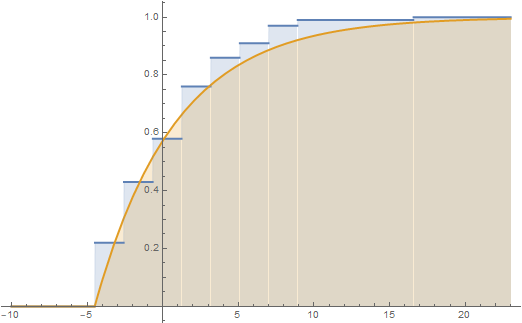
\includegraphics{FF}
  \caption{Рис. 4. Емпірична функція розподілу у порівнянні з відповідною функцією розподілу.}
\end{center}
\begin{center}
  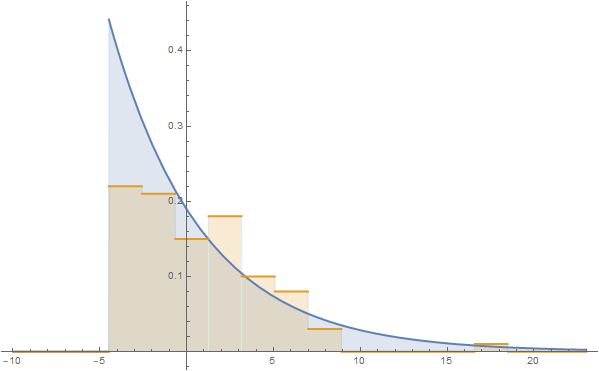
\includegraphics[scale=0.9]{fH}
  \caption{Рис. 5. Гістограма у порівнянні із відповідною функцією щільності.}
\end{center}
Тоді альтернативною гіпотезою буде $H_1=\left\{\xi\nsim Exp(\lambda,a)\right\}$.

\newpage
\section{Оцінка параметрів.}

Для зміщеного експоненційного розподівлу маємо параметри $\lambda$ та $a$. Треба їх оцінити.\\\\
\quad\underline{\textbf{Метод моментів.}}\\

Для знаходження оцінки методом моментів, треба розв'язати систему рівнянь, що включає s моментів розподілу, де s~--~кількість параметрів розподілу, а також їх емпіричні еквіваленти.\\
$$\E \xi=\int\limits_{-\infty}^{+\infty}{xf_\xi(x)\,dx}=
\int\limits_{a}^{+\infty}{x\cdot\frac1\lambda e^{-\frac{x-a}\lambda}\,dx}=
\frac1\lambda\int\limits_{a}^{+\infty}{xe^{-\frac{x-a}\lambda}\,dx}=$$
$$=\left|\begin{array}{cc}
  u=x; & dv=e^{-\frac{x-a}\lambda}\,dx\\
  du=dx; & v=-\lambda e^{-\frac{x-a}\lambda}
\end{array}\right|=
\frac1\lambda\left(
\left.-\lambda xe^{-\frac{x-a}\lambda}\right|_a^{+\infty}+
\lambda \int\limits_{a}^{+\infty}{e^{-\frac{x-a}\lambda}\,dx}
\right)=$$
\be=\frac1\lambda\left(
0-\left(-\lambda a\right)-
\left.\lambda^2e^{-\frac{x-a}\lambda}\right|_a^{+\infty}
\right)=
\frac1\lambda\left(
\lambda a -\lambda^2\left(0-1\right)
\right)=\fbox{$a+\lambda$}\,;\ee
$$\E \xi^2= \int\limits_{-\infty}^{+\infty}{
x^2\cdot f_\xi(x)\,dx}=
\frac1\lambda\int\limits_{a}^{+\infty}{x^2e^{-\frac{x-a}\lambda}\,dx}=
\left|\begin{array}{cc}
  u=x^2; & dv=e^{-\frac{x-a}\lambda}\,dx\\
  du=2x\,dx; & v=-\lambda e^{-\frac{x-a}\lambda}
\end{array}\ringh|=$$
$$\frac1\lambda\left(
\left.-\lambda x^2e^{-\frac{x-a}\lambda}\right|_a^{+\infty}+
2\lambda\int\limits_{a}^{+\infty}{xe^{-\frac{x-a}\lambda}\,dx}
\right)=
\frac1\lambda\left(
\lambda a^2+2\lambda\left(\lambda a+\lambda^2\right)
\right)=$$
\be=a^2+2\lambda a+2\lambda^2 = \fbox{$\left(a+\lambda\right)^2+\lambda^2$}\ee\\
Отримуємо наступну систему рівнянь:\\
$$\left\{\begin{array}{l}
  a^*+\lambda^*=\overline{\xi}\\
  (a^*+\lambda^*)^2+(\lambda^*)^2=\overline{\xi^2}
\end{array}\right.$$\\
\be\left\{\begin{array}{l}
  \lambda^*=\sqrt{\overline{\xi^2}-\overline{\xi}^2}\approx3.0174\\
  a^*=\overline{\xi}-\sqrt{\overline{\xi^2}-\overline{\xi}^2}\approx-2.2236
\end{array}\right.\ee

\newpage
\underline{\textbf{Метод максимальної вірогідності.}}\\

Для знаходження оцінки методом максимальної вірогідності треба максимізувати функцію вірогідності за параметрами $\lambda$ та $a$. Можемо спробувати знайти її глобальний максимум.
$$\mathcal{L}(x_1,\dots,x_n,\lambda,a)=f_{\xi_1,\dots,\xi_n}(x_1,\dots,x_n)=\prod\limits_{i=1}^n{f_{\xi_i}(x_i)}=\prod\limits_{i=1}^n{f_\xi(x_i)}=$$
$$=\arrowvert x\geq a\arrowvert=\prod\limits_{i=1}^n{\frac1\lambda e^{-\frac{x_i-a}\lambda}}=
\frac1{\lambda^n}e^{-\frac1\lambda(x_1+\dots+x_n-na)}$$
Для легшого обчислення похідних варто використати функцію логарифма, оскільки вона монотонно зростаюча, а логарифм добутку родівнює сумі логарифмів множників, що спрощує диференціювання.
$$\ln{\mathcal{L}}=-n\ln{\lambda}-\frac{x_1+\dots+x_n-na}\lambda$$
Знайдемо часткові похідні першого та другого порядків за параметрами:
$$\frac{\partial\ln{\mathcal{L}}}{\partial\lambda}=
-\frac{n}\lambda+\frac{x_1+\dots+x_n-na}{\lambda^2}=
\frac{x_1+\dots+x_n-na-n\lambda}{\lambda^2}\,;$$
$$\frac{\partial\ln{\mathcal{L}}}{\partial a}=\frac{n}\lambda\,;$$\\
$$\frac{\partial^2\ln{\mathcal{L}}}{\partial \lambda^2}=
\frac{n}{\lambda^2}-2\frac{x_1+\dots+x_n-na}{\lambda^3}\,;$$
$$\frac{\partial^2\ln{\mathcal{L}}}{\partial a^2}=0\,;$$
$$\frac{\partial^2\ln{\mathcal{L}}}{\partial \lambda\partial a}=-\frac{n}{\lambda^2}\,;$$\\
$$\det{\left(\begin{array}{cc}
  \frac{\partial^2\ln{\mathcal{L}}}{\partial \lambda^2} &
  \frac{\partial^2\ln{\mathcal{L}}}{\partial \lambda\partial a}\\\\
  \frac{\partial^2\ln{\mathcal{L}}}{\partial \lambda\partial a} &
  \frac{\partial^2\ln{\mathcal{L}}}{\partial a^2}
\end{array}\right)}=0-\left(-\frac{n}{\lambda^2}\right)^2<0$$
Отже функція не має екстремумів, тому принаймні спробуємо максимізувати її значення.
\\
\be
\left\{\begin{array}{l}
  \frac{\partial\ln\mathcal{L}}{\partial\lambda^*}=0\,;\\\\
  \frac{\partial\ln\mathcal{L}}{\partial a^*}=0\,.
\end{array}\right.\quad\Rightarrow\quad
\left\{\begin{array}{l}
  a^*+\lambda^*=\overline{x};\\
  \lambda^*\ne0;\\
  \lambda^*\rightarrow\infty\,.
\end{array}\right.\quad\Rightarrow\quad
\left\{\begin{array}{l}
  a^* = \min\{x_i\}=-4.49\,;\\
  \lambda^*=\overline{x}-a^*=5.2838\,.
\end{array}\right.
\ee

\newpage
\section{Дослідження оцінки.}

Кращою з двох отриманих оцінок є оцінка методом максимальної вірогідності. Проведемо її дослідження.\\
\underline{\textbf{Незміщеність.}}\\
$$\E {a^*}=\E {\min\{\xi_i\}}\fbox{$=$}$$
Щільність розподілу мінімума:
$$f_\xi(x)=\frac1\lambda e^{-\frac{x-a}\lambda}\cdot\mathbb{I}\{x\geq a\};\quad
F_\xi(x)=(1-e^{-\frac{x-a}\lambda})\cdot\mathbb{I}\{x\geq a\}$$
$$f_{\min\{\xi\}}(x)=n(1-F_\xi(x))^{n-1}f_\xi(x)=
\frac{n}\lambda e^{-n\frac{x-a}{\lambda}}\cdot\mathbb{I}\{x\geq a\}$$
$$\fbox{$=$}\int\limits_{a}^{+\infty}{x\cdot\frac{n}\lambda e^{-n\frac{x-a}{\lambda}}\,dx}=
\left|\begin{array}{cc}
  u=x; & dv=e^{-n\frac{x-a}{\lambda}}\,dx\\
  du=dx; & v=-\frac{\lambda}{n}e^{-n\frac{x-a}{\lambda}}
\end{array}\right|=$$
$$\frac{n}{\lambda}\left(\left.-\frac{\lambda}{n}xe^{-n\frac{x-a}{\lambda}}\right|_a^{+\infty}+\frac{\lambda}{n}\int\limits_{a}^{+\infty}{e^{-n\frac{x-a}{\lambda}}\,dx}\right)=
a-\left.\frac{\lambda}{n}e^{-n\frac{(x-a)}{\lambda}}\right|_a^{+\infty}=
\frac{na+\lambda}n\ne a\Rightarrow$$
\be\Rightarrow a^*\text{~--~не є незміщеною.}\ee
$$\lim\limits_{n\to\infty}{\E a^*}=\lim\limits_{n\to\infty}{\frac{na+\lambda}n}=a\Rightarrow$$
\be\Rightarrow a^*\text{~--~є асимптотично незміщеною.}\ee
\\
$$\E \lambda^*=\E \left(\overline{\xi}-a^*\right)=
\E \frac{\xi_1+\dots+\xi_n}n-\frac{na+\lambda}n=
\frac1nn\E \xi_i-\frac{na+\lambda}n=$$
$$a+\lambda-\frac{na+\lambda}n=\frac{n\lambda-\lambda}n\ne\lambda\Rightarrow$$
\be\Rightarrow\lambda^*\text{~--~не є незміщеною.}\ee
$$\lim\limits_{n\to\infty}{\E \lambda^*}=\lim\limits_{n\to\infty}{\frac{n\lambda-\lambda}n}=\lambda\Rightarrow$$
\be\Rightarrow\lambda^*\text{~--~є асимптотично незміщеною.}\ee
\newpage\\
\underline{\textbf{Консистентність.}}
$$\mathbb{P}\lim\limits_{n\to\infty}{a^*}\stackrel{?}{=}a$$
$$\mathbb{P}\lim\limits_{n\to\infty}{\lambda^*}\stackrel{?}{=}\lambda$$
Перевіримо за лемою про консистентність. Для цього потрібно обчислити дисперсії оцінок.
$$\D a^*=\E (a^*)^2-\left(\E a^*\right)^2\,;$$
$$\E (a^*)^2=\frac{n}\lambda\int\limits_{a}^{+\infty}{x^2\cdot e^{-n\frac{x-a}\lambda}\,dx}=
\left|\begin{array}{cc}
  u=x^2; & dv=e^{-n\frac{x-a}\lambda}\,dx\\
  du=2x\,dx; & v=-\frac\lambda{n}e^{-n\frac{x-a}\lambda}
\end{array}\right|=$$
$$=\left.-x^2e^{-n\frac{x-a}\lambda}\right|_a^{+\infty}+2\int\limits_{a}^{+\infty}{xe^{-n\frac{x-a}\lambda}\,dx}=
a^2+2\left(\left.-\frac{\lambda}{n}xe^{-n\frac{x-a}{\lambda}}\right|_a^{+\infty}+
\frac{\lambda}{n}\int\limits_{a}^{+\infty}{e^{-n\frac{x-a}{\lambda}}\,dx}\right)=$$
$$=a^2+2\cdot\frac{\lambda}n\cdot\frac{na+\lambda}n=
a^2+\frac{2na\lambda+2\lambda^2}{n^2}\,;$$
\be\D a^*=a^2+\frac{2na\lambda+2\lambda^2}{n^2}-\frac{(na+\lambda)^2}{n^2}=\frac{\lambda^2}{n^2}\,;\ee
$$\left\{\begin{array}{l}
  \lim\limits_{n\to\infty}{\D a^*}=a^2+0-a^2=0\,;\\
  a^*\text{~--~асимптотично незміщена.}
\end{array}\right.\Rightarrow$$
\be\Rightarrow a^*\text{~--~консистентна}\ee\\

$$\D \lambda^*=\D (\overline{\xi}-a^*)=
\D \overline{\xi}+\D a^*=\D\frac{\xi_1+\dots+\xi_n}n+\D a^*=
\frac1{n^2}\D(\xi_1+\dots+\xi_n)+\D a^*=$$
$$=\frac1n\D\xi_i+\D a^*=
\frac1n\left(\E{\xi^2}-\left(\E\xi\right)^2\right)+\D a^*=
\frac1n\left(\cancel{(a+\lambda)^2}+\lambda^2-\cancel{(a+\lambda)^2}\right)+\frac{\lambda^2}{n^2}=$$
\be=\frac{(n+1)\lambda^2}{n^2}\ee
$$\left\{\begin{array}{l}
  \lim\limits_{n\to\infty}{\D\lambda^*}=\lim\limits_{n\to\infty}{\frac{(n+1)\lambda^2}{n^2}}=0\,;\\
  \lambda^*\text{~--~асимптотично незміщена.}
\end{array}\right.\Rightarrow$$
\be\Rightarrow\lambda^*\text{~--~консистентна.}\ee

\newpage
\underline{\textbf{Ефективність.}}\\
\justifying{Оскільки оцінки виявилися зміщеними, перевіряти їх на ефективність немає сенсу.}

\newpage
\section{Інтервальні оцінки параметрів.}
\underline{Задача:} побудувати інтервальні оцінки параметрів розподілу з довірчою імовірністю $\gamma=0.95$.\\
Оскільки розподіл нестандартний, доволі важко буде знайти точний довірчий інтервал, але при великих n доволі непоганої точності можна досягти і з використанням асимптотичних довірчих інтервалів, тому знайдемо саме такий інтервал.\\
\textbf{Озн.} $(\theta^*_{1n},\theta^*_{2n})$ називається асимптотичним довірчим інтервалом для параметру $\theta$, якщо $\lim\limits_{\overline{n\to\infty}}{\mathbb{P}\{\theta^*_{1n}<\theta<\theta^*_{2n}\}} \stackrel{(\geq)}{=}\gamma$.\\
\\При великих $n$
$$\frac{\theta^*-\E\theta^*}{\sqrt{\D\theta^*}}\approx\mathcal{N}(0,1)$$
% \begin{tikzpicture}
%   \begin{axis}[
%     axis lines=middle,
%     xmin = -5, xmax = 5,
%     ymin = -.05, ymax = .5,
%     %xtick distance = 2.5,
%     %ytick distance = 0.5,
%     grid = both,
%     minor tick num = 1,
%     major grid style = {lightgray},
%     width = \textwidth,
%     height = 0.5\textwidth]
%     \addplot[
%       domain = -5:5,
%       samples = 200,
%       smooth,
%       thick,
%       blue,
%       name path=A
%     ] {1/sqrt(2*pi)*exp(-x^2/2)};
%     \addplot[smooth,red] coordinates {(-2.3,-0.01)(-2.3,0.05)};
%     \addplot[smooth,red] coordinates {(2.3,-0.01)(2.3,0.05)};
%     \path[name path=xaxis] (\pgfkeysvalueof{/pgfplots/xmin}, 0) -- (\pgfkeysvalueof{/pgfplots/xmax},0);
%     \addplot[red, pattern=north west lines] fill between[of=A and xaxis, soft clip={domain=-2.3:2.3}];
%   \end{axis}
% \end{tikzpicture}
\begin{center}
  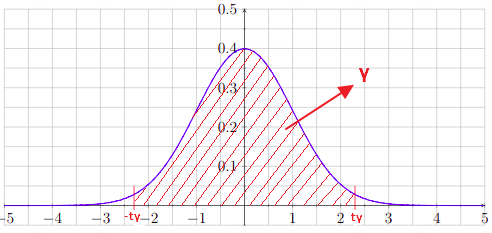
\includegraphics{N(0,1)}
  \caption{Рис. 6. Стандартний нормальний розподіл.}
\end{center}
\be t_\gamma:\Phi(t_\gamma)=\frac\gamma{2}\ee
$$\mathbb{P}\{-t_\gamma<\mathcal{N}(0,1)<t_\gamma\}=\gamma$$
\be\mathbb{P}\{-t_\gamma<\frac{\theta^*-\E\theta^*}{\sqrt{\D\theta^*}}<t_\gamma\}=\gamma\ee
Для знаходження асимптотичної інтервальної оцінки параметра $\theta$ потрібно розв'язати нерівніть під оператором $\mathbb{P}$ відносно $\theta$.\\
Для $\gamma=0.95$ маємо значення $t_\gamma=1.95996$.

\newpage
\underline{\textbf{Асимптотичний інтервал для параметра зміщеного середнього $\lambda$.}}\\

Оскільки для даної оцінки рахувати дисперсію потрібно через коваріацію, бо її компоненти залежні, то можна спробувати трохи знизити точніть, але спростити обчислення~--~прийняти $a^*$ відомим, підставивши оцінене раніше обчислену оцінку ММВ.
$$\frac{\lambda^*-\E\lambda^*}{\sqrt{\D\lambda^*}}=
\left|\begin{array}{c}
  \D\lambda^*=\D(\overline{\xi}-a)=\D\overline{\xi}=\frac1n\D\xi_i=\frac1n\D\xi=\\
  =\frac1n\left(\E\xi^2-(\E\xi)^2\right)=\frac1n\left((a+\lambda)^2+\lambda^2-(a+\lambda)^2\right)=\frac{\lambda^2}n
\end{array}\right|=$$
$$=\frac{\lambda^*-\frac{(n-1)\lambda}n}{\lambda}\sqrt{n}=
\frac{n\lambda^*-(n-1)\lambda}{n\lambda}\sqrt{n}=
\frac{n\lambda^*-(n-1)\lambda}{\sqrt{n}\lambda}\,;$$
$$-t_\gamma<\frac{n\lambda^*-(n-1)\lambda}{\sqrt{n}\lambda}<t_\gamma\quad\Rightarrow\quad
\frac{(n\lambda^*-(n-1)\lambda)^2}{n\lambda^2}<t_\gamma^2\Rightarrow$$
$$\Rightarrow(n-1)^2\lambda^2-2(n^2-n)\lambda^*\lambda+n^2(\lambda^*)^2<nt_\gamma^2\lambda^2\Rightarrow$$
$$\Rightarrow(n-nt_\gamma^2-1)\lambda^2-2(n^2-n)\lambda^*\lambda+n^2(\lambda^*)^2<0\;\fbox{\Rightarrow}$$
$$\mathcal{D}=b^2-4\hat{a}c=4(n^2-n)^2(\lambda^*)^2-4(n-nt_\gamma^2-1)n^2(\lambda^*)^2=$$
$$=4n^4(\lambda^*)^2
-8n^3(\lambda^*)^2 % 12
+4n^2(\lambda^*)^2
-4n^3(\lambda^*)^2 %----
+4n^3t_\gamma^2(\lambda^*)^2
+4n^2(\lambda^*)^2=$$
$$=4n^4(\lambda^*)^2
-12n^3(\lambda^*)^2
+8n^2(\lambda^*)^2
+4n^3t_\gamma^2(\lambda^*)^2=$$
$$=4n^2(\lambda^*)^2(n^2-3n+2+nt_\gamma^2)\,;$$
$$\fbox{\Rightarrow}\;\lambda^*_{1,2}=\frac{-b\pm\sqrt{\mathcal{D}}}{2\hat{a}}=
\frac{(n^2-n)\lambda^*\pm n\lambda^*\sqrt{n^2-3n+2+nt_\gamma^2}}{n-nt^2_\gamma-1}=$$
\be=\frac{n\lambda^*\left((n-1)\pm\sqrt{n^2-3n+2+nt_\gamma^2}\right)}{n-nt_\gamma^2-1}\ee


\newpage
\underline{\textbf{Асимптотичний інтервал для параметра зміщення $a$.}}\\
$$\frac{a^*-\E a^*}{\sqrt{\D a^*}}=
\frac{\min\{\xi_i\}-\frac{na+\lambda}{n}}{\frac{\lambda}n}=
\frac{n}\lambda\min\{\xi_1\}-\frac{na}\lambda-1\,;$$
$$-t_\gamma<\frac{n}\lambda\min\{\xi_1\}-\frac{na}\lambda-1<t_\gamma\Rightarrow$$
$$\Rightarrow-t_\gamma-\frac{n}\lambda\min\{\xi_1\}+1<
-\frac{na}\lambda<
t_\gamma-\frac{n}\lambda\min\{\xi_1\}+1\Rightarrow$$
$$\Rightarrow\frac{\lambda t_\gamma}n+\min\{\xi_i\}-\frac\lambda{n}
>a>
-\frac{\lambda t_\gamma}n+\min\{\xi_i\}-\frac\lambda{n}\,;$$
\be a\in\left(
-\frac{\lambda t_\gamma}n+\min\{\xi_i\}-\frac\lambda{n},\quad
\frac{\lambda t_\gamma}n+\min\{\xi_i\}-\frac\lambda{n}
\right)\ee
Оскільки ми не маємо точного значення параметра $\lambda$, також можемо взяти його оцінку, що знизить точність, але інтервал і так був асимптотичним, тому це не сильно вплине. Отже:
$$a\in\left(-\frac{\lambda^*t_\gamma}n+\min\{x_i\}-\frac{\lambda}n,\quad
\frac{\lambda^*t_\gamma}n+\min\{x_i\}-\frac{\lambda}n\right)=$$
$$=(-4.6464,\quad-4.4393).$$
Як видно, отримана методом максимальної вірогідності оцінка потрапляє у заданий проміжок, однак оцінка методом моментів~--~ні.



\end{document}
